\subsection{Distance to Planes}

Let's first consider the distance between a point and a plane. If the point is on the plane, then the distance is zero. Otherwise, the distance between the point and the plane will be the shortest distance between the point and the plane. This can be found by starting at the plane, and traveling towards the plane parallel to the normal vector of the plane.

\begin{center}
    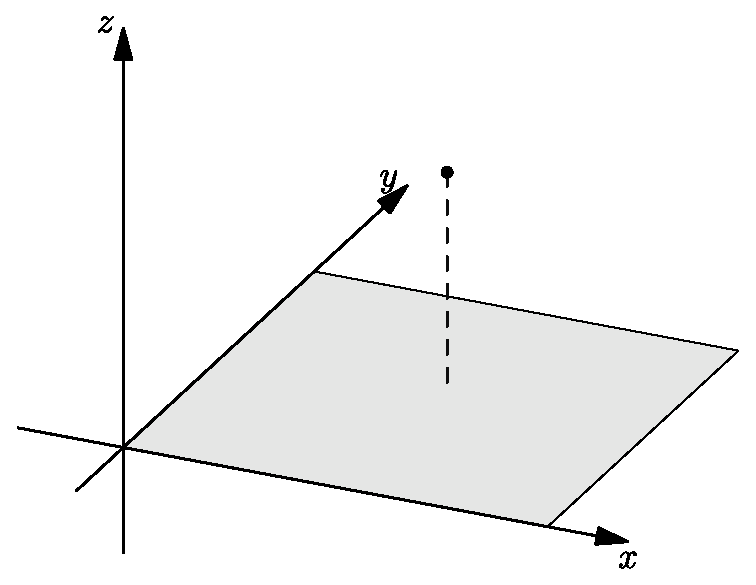
\includegraphics[width=300pt]{Figures/PlanetoDot}\\
    Point to Plane in $\bbr^3$
\end{center}

So if we could just find the point in the plane that is directly ``beneath" our point, then we'd be set. Unfortunately, that's actually really really hard. Fortunately, we don't have to do that.

\begin{exercise}{Point to Plane}
Lets let our plane be the plane $z=0$. Note that this is literally the $xy$-plane. Let's let our point be $(2,1,3)$. Even though it's not hard here to figure out what the point directly below $(2,1,3)$ is, we're gonna assume that we can't. So instead, let's pick a random point on that plane. Like $(4,2,0)$.
\begin{center}
    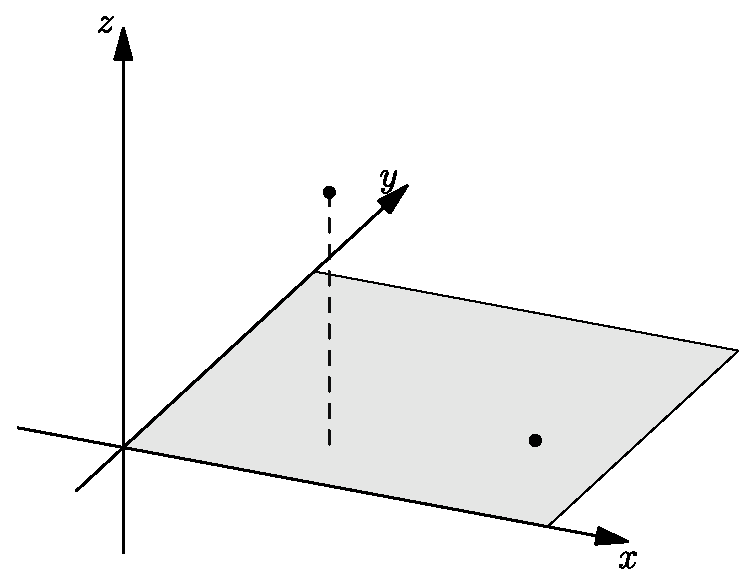
\includegraphics[width=300pt]{Figures/pointplaneex1}\\$(2,1,3)$ and $(4,2,0)$.
\end{center}
\vspace{1em}
\begin{enumerate}
\item Find the vector that goes from $(4,2,0)$ to $(2,1,3)$. Call that vector $\vcv$.
\vspace{1em}
\end{enumerate}
Well, why would we find that vector? It's certainly not the shortest distance between our point and our plane. But if we look at that vector between our two points, you may notice something.
\vspace{1em}
\begin{center}
    \includegraphics[width=300pt]{Figures/pointplaneex2}\\\href{https://www.geogebra.org/3d/kdsbfgck}{The vector from $(4,2,0)$ to $(2,1,3)$ (Geogebra Link).}
\end{center}
\vspace{1em}
While the length of $\vcv$ is not the distance we are looking for, if we were to find the component of $\vcv$ in the direction perpendicular to our plane, that would, in fact, be the right length. And that's \textit{exactly} what our vector projection is.
\vspace{1em}
\begin{enumerate}
\item[2.] Find $\vcn$, the normal vector for our plane $z=0$.
\vspace{1em}
\item[3.] Find $\proj{\vcv}{\vcn}$, the projection of $\vcv$ onto $\vcn$, and the distance between our point and our plane.
\vspace{1em}
\item[4.] Take the magnitude of the projection you just found. That is, find $|| \proj{\vcv}{\vcn}||$.
\end{enumerate}
\end{exercise}

\begin{claim}{Point to Plane Algorithm}
To find the distance between a point $P$ and a plane:
\vspace{1em}
\begin{enumerate}
\item Pick an arbitrary point, $Q$, on the plane.
\vspace{1em}
\item Find the vector difference between $P$ and $Q$, call that $\vcv$.
\vspace{1em}
\item Find the normal vector for your plane, call that $\vcn$.
\vspace{1em}
\item Find $\proj{\vcv}{\vcn}$, or the projection of $\vcv$ onto $\vcn$.
\vspace{1em}
\item Find $||\proj{\vcv}{\vcn}|| $. This is the distance required.
\end{enumerate}
\end{claim}

So let's now look at the distance between two planes! First, note that if two planes intersect, then they share a point, so the distance between the two planes must be zero. The only way for planes to not intersect is if they are \textit{parallel}. 

\begin{center}
    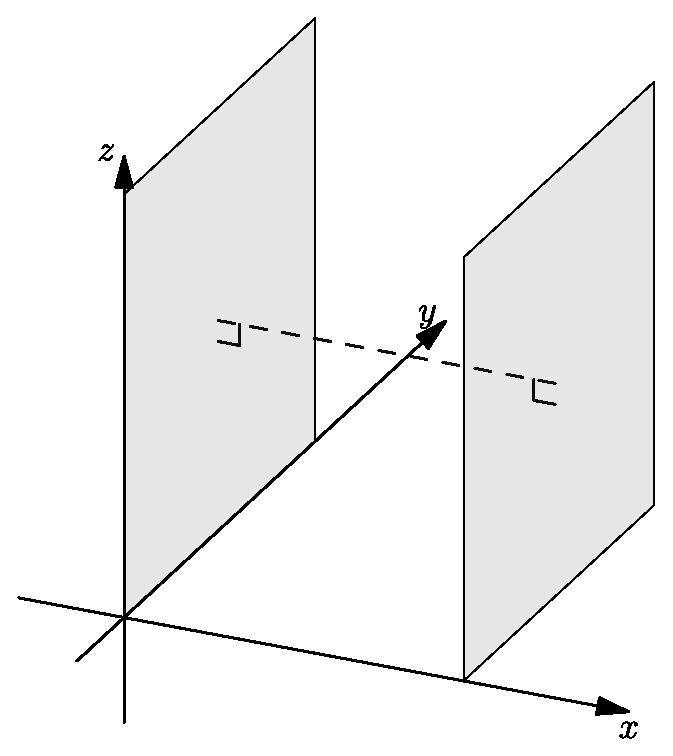
\includegraphics[width=300pt]{Figures/PlanetoPlane}\\
    Parallel Planes in $\bbr^3$
\end{center}

\begin{claim}{Plane to Plane Algorithm}
To find the distance between two planes:
\vspace{1em}
\begin{enumerate}
\item Pick an arbitrary point, $P$ on one of your planes.
\vspace{1em}
\item Execute the Point to Plane algorithm with the chosen $P$ and the other plane.
\end{enumerate}
\end{claim}

\begin{exercise}{Plane to Plane}
Find the distances between the following planes.
\vspace{1em}
\begin{enumerate}
\item Find the distance between \href{https://www.geogebra.org/3d/gn8etvbp}{$2x-y+z=2$ and $2x-y+z=-1$. (Geogebra Link)}
\vspace{1em}
\item Find the distance between \href{https://www.geogebra.org/3d/ekksyyew}{$5x-2y+z=6$ and $5x-2y+z=-3$. (Geogebra Link)}
\end{enumerate}
\end{exercise}

Similarly, the distance between a line and a plane also quickly reduces. If the line intersects the plane, then the distance is 0, but if the line is parallel to the plane, then you pick any point on the line and then use the point to plane algorithm.

\begin{claim}{Line to Plane Algorithm}
To find the distance between a line and a plane:
\vspace{1em}
\begin{enumerate}
\item Pick an arbitrary point, $P$ on your line.
\vspace{1em}
\item Execute the Point to Plane algorithm with the chosen $P$ and the plane.
\end{enumerate}
\end{claim}

\begin{exercise}{Line to Plane}
Find the distances between the following Lines and Planes.
\vspace{1em}
\begin{enumerate}
\item Find the distance between \href{https://www.geogebra.org/3d/guykkgyr}{$2x+y-z=3$ and $\dfrac{x}{2}=\dfrac{y-1}{2}=\dfrac{z}{6}$. (Geogebra Link)}
\vspace{1em}
\item Find the distance between $2x+y-z=3$ and $\dfrac{x}{2}=\dfrac{y-1}{4}=\dfrac{z}{6}$. Hint: is this line parallel to the plane? Check by taking the dot product of the normal vector of the plane and the direction vector of the line.
\end{enumerate}
\end{exercise}